\documentclass[11pt]{article}

%  Overall look
\usepackage[margin=0.54in]{geometry}  

% Greek
\usepackage{alphabeta}
\usepackage[utf8]{inputenc}
\usepackage[greek, english]{babel}


% Figures
\usepackage{graphicx}
\usepackage{caption}
\usepackage{subcaption}
\usepackage{float}


% Tables
\usepackage{multirow}
\usepackage{multicol}
\usepackage{booktabs}


% Math
\usepackage{amsmath}
\usepackage{amssymb}
\usepackage{mathtools}
\usepackage{wasysym}
\usepackage{steinmetz}
\usepackage{cancel}
\usepackage{bigints}
\newcommand{\eqdoub}{\overset{\mathrm{}}{=\joinrel=}}
\newcommand{\eqsix}{\overset{\mathrm{}}{=\joinrel=\joinrel=\joinrel=\joinrel=\joinrel=\joinrel}}
\newcommand{\eqeight}{\overset{\mathrm{}}{=\joinrel=\joinrel=\joinrel=\joinrel=\joinrel=\joinrel=\joinrel=}}


%code
\usepackage{listings}
\usepackage{color} %red, green, blue, yellow, cyan, magenta, black, white
\definecolor{mygreen}{RGB}{28,172,0} % color values Red, Green, Blue
\definecolor{mylilas}{RGB}{170,55,241}
\lstset{language=Matlab,%
	basicstyle=\small, %or \small or \footnotesize etc.
	breaklines=true,%
	frame=single,
	mathescape,
	morekeywords={matlab2tikz},
	keywordstyle=\color{blue},%
	morekeywords=[2]{1}, 
	keywordstyle=[2]{\color{black}},
	identifierstyle=\color{black},%
	stringstyle=\color{mylilas},
	commentstyle=\color{mygreen},%
	showstringspaces=false,%without this there will be a symbol in the places where there is a space
	emph=[1]{for,end,break,on,off},emphstyle=[1]\color{red}, %some words to emphasise
	numberstyle={\tiny \color{black}},% size of the numbers
	numbersep=9pt, % this defines how far the numbers are from the text
}


% For drawing
\usepackage{tikz}
\usetikzlibrary{arrows,automata,calc,shapes,backgrounds}
\usetikzlibrary{positioning} 	% For left right etc
\tikzset{
	treenode/.style = {align=center, inner sep=0pt, text centered,
		font=\sffamily},
	arn/.style = {treenode, circle, black, font=\sffamily\bfseries, draw=black,
		fill=white, text width=4.1ex},
	arnrec/.style = {treenode, rectangle, black, font=\sffamily\bfseries, draw=black,
		fill=white, text width=7.5ex,minimum width=4.0ex, minimum height=4.0ex},
	arnsmall/.style = {treenode, circle, black, font=\sffamily\bfseries, draw=black,
		fill=white, text width=1.5ex},
}
\usepackage{xcolor}
\definecolor{purple}{HTML}{9B26B6}
\usetikzlibrary{arrows.meta}
\usetikzlibrary{matrix,positioning}

% Table of contents
% Clickable
\usepackage{hyperref}
\hypersetup{
	colorlinks,
	citecolor=black,
	filecolor=black,
	linkcolor=black,
	urlcolor=black
}
% Dots
\usepackage{tocloft}
\renewcommand{\cftsecleader}{\cftdotfill{\cftdotsep}}


%First page
\newcommand{\subject}{Ηλεκτρονικά Ισχύος}
\newcommand{\descript}{3η Άσκηση}
\newcommand{\names}{Δούνης Λουκάς\\
                    Ζαφειράκης Κωνσταντίνος\\
                    Σταυρόπουλος Αλέξανδρος Ανδρέας 2019030109}
\newcommand{\lecturer}{Φώτιος Κανέλλος}
\newcommand{\lablecturer}{Δήμητρα Κυριακού}
\newcommand{\term}{Εαρινό εξάμηνο 2022-2023}


% Line above page numbering
\usepackage{titleps}%
\newpagestyle{ruled}{%
	\footrule
	\setfoot{}{\thepage}{}}
\pagestyle{ruled}



% Begin Code
\begin{document}
	\begin{titlepage}
	\begin{center}
		\vspace*{1cm}
		\rule{\textwidth}{1.6pt}\vspace*{-\baselineskip}\vspace*{2pt}
		\rule{\textwidth}{0.4pt}\\[\baselineskip]
		{\LARGE{\textbf{\subject}}}\\
		\vspace{0.3cm}
		{\large\descript\\}
		\rule{\textwidth}{0.4pt}\vspace*{-\baselineskip}\vspace{3.2pt}
		\rule{\textwidth}{1.6pt}\\[\baselineskip]
				
		\vspace{1.5cm}
		\textbf{\names}
		\vspace{0.3cm}
		
		\vfill
		
		Διδάσκων:\\
		\lecturer\\
		\vspace{0.5cm}
		Υπεύθυνος εργαστηρίου:\\
        
		\lablecturer
		\vspace{0.8cm}
		
		
\includegraphics[width=0.3\textwidth]{Images/university}
		
		ΗΜΜΥ\\
		Πολυτεχνείο Κρήτης\\
		\term
		
	\end{center}
\end{titlepage}
	\newpage
	% Remaning and Centering ToC
	\begin{center}
		\renewcommand{\contentsname}{\centering \text{Πίνακας Περιεχομένων}}
		\tableofcontents{\protect\thispagestyle{empty}}
	\end{center}
    \newpage
    \setcounter{page}{1}
    \section{Περιγραφή Λειτουργίας Αντιστροφέων}

\subsection{Μονοφασικός Αντιστροφέας}
\noindent
Ο μονοφασικός Αντιστροφέας αποτελεί μία συσκευή η οποία μετατρέπει DC τάση και ρεύμα σε AC. Το κύκλωμα κατασκευάζεται από τέσσερεις ελεγχόμενους διακόπτες και τέσσερεις διόδους συνδεδεμένες ως εξής:
\begin{figure}[H]
	\centering
	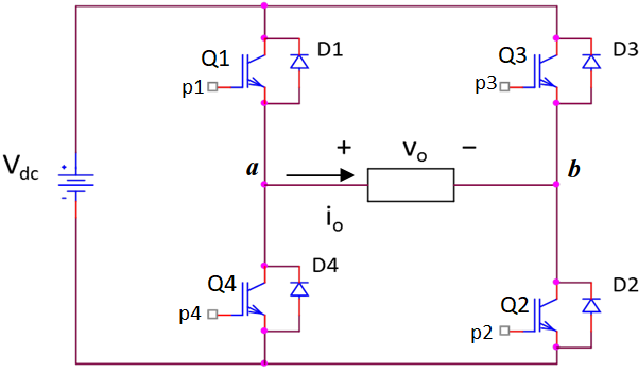
\includegraphics[width=0.45\textwidth]{Images/circuit1.png}
	\label{circuit_1}
\end{figure}

\subsubsection{Μονοφασικός Αντιστροφέας Γέφυρας Τετραγωνικού Παλμού}
\subsubsection{Μονοφασικός Αντιστροφέας Γέφυρας με μονοπολική PWM}
\label{single_PWM}

\noindent
Για την παραγωγή της AC τάσης και AC ρεύματος εξόδου, σε αυτή την περίπτωση, δημιουργούνται τετραγωνικοί παλμοί διαφορετικού εύρους μέσω των οποίων, ανάλογα με το εύρος τους, ελέγχεται το πλάτος της τάσης εξόδου.
\noindent\\\\\\
Στην παραπάνω διάταξη τα transistor ενεργοποιούνται με συγκεκριμένο σειρά ώστε οι παλμοί ελέγχου να κατασκευάζουν την επιθυμητή τάση εξόδου εξόδου, ενώ οι δίοδοι χρησιμοποιούνται  για την ροή ρεύματος προς αντίθετη φορά από αυτή των ενεργοποιημένων transistor, λόγω της εναλλασσόμενης μορφής του ρεύματος.

\noindent\\
Για την παραγωγή των παλμών ελέγχου, κατασκευάζεται το επιθυμητό ημιτονοειδές σήμα εξόδου καθώς και ένας τριγωνικός παλμός (Φέρον) πλάτους $V_{dc}$, συχνότητας ίση με την διακοπτική $(m_f \cdot f)$. Συγκρίνοντας το φέρον με το θετικό ημίτονο εξόδου προκύπτουν οι παλμοί ελέγχου των transistor $Q_1$, $Q_4$ ενώ συγκρίνοντάς το με το αρνητικό προκύπτουν οι παλμοί ελέγχου των transistor $Q_2$, $Q_3$, όπως αυτοί φαίνονται στον πίνακα που ακολουθεί:
\begin{table}[h]
	\centering
	\begin{tabular}{ccccc}
		Condition                                     & $Q_1$ & $Q_2$ & $Q_3$ & $Q_4$ \\ \hline
		\multicolumn{1}{c|}{$V_{ref} > V_{carrier}$}  & ON    & -     & -     & OFF   \\
		\multicolumn{1}{c|}{$V_{ref} < V_{carrier}$}  & OFF   & -     & -     & ON    \\
		\multicolumn{1}{c|}{$-V_{ref} > V_{carrier}$} & -     & OFF   & ON    & -     \\
		\multicolumn{1}{c|}{$-V_{ref} < V_{carrier}$} & -     & ON    & OFF   & -    
	\end{tabular}
\end{table}
\noindent\\
Σύμφωνα με τα παραπάνω δεδομένα προκύπτει η τιμή της τάσης στο κόμβο a και στον κόμβο b, εφόσον τα ενεργά transistor δρουν ως βραχυκύκλωμα. Μέσω των τάσεων $V_a$ και $V_b$ η τάση εξόδου στο φορτίο:
\begin{equation}
	V_{out} = V_a - V_b
\end{equation}
\noindent
Τέλος, για την καλύτερη ανάλυση του συστήματος ορίζεται ο δείκτης διαμόρφωσης πλάτους ($m_a$) και ο δείκτης διαμόρφωσης συχνότητας ($m_f$). Ο  $m_a$ ορίζεται ως το πηλίκο μεταξύ του πλάτους του σήματος αναφοράς και του πλάτους του φέροντος και σύμφωνα με την θεωρία, για τιμές μικρότερες της μονάδας επηρεάζει το πλάτης της βασικής αρμονικής ως εξής:
\begin{equation}
	V_1 = m_a \cdot V_{dc}
\end{equation}
Αντίστοιχα, ο $m_f$ ορίζεται ως το πηλίκο μεταξύ της συχνότητας του σήματος αναφοράς και της συχνότητας του φέροντος και σύμφωνα με την θεωρία, αυξάνοντας τον οι αρμονικές του σήματος μετατοπίζονται σε μεγαλύτερες συχνότητες.
    \section{Κανονικές Εκφράσεις}

\subsection[Ερώτημα α]{\textbf{α) }} L = \{w $\in \{a, b\}^*$ : η w περιέχει ακριβώς 2 εμφανίσεις του a και άρτιο αριθμό από b\}
\begin{equation*}
	L = \mathcal{L} \Bigg( (bb)^* \bigg( \Big( (ab \cup ba) (bb)^*(ab \cup ba) \Big)  \bigcup    \Big(aa\Big)  \bigg) (bb)^*\Bigg)
\end{equation*}

\subsection[Ερώτημα β]{\textbf{β) }} L = \{w $\in {a, b}^*$ : η w αρχίζει και τελειώνει με το ίδιο σύμβολο και έχει περιττό μήκος\}
\begin{equation*}
	L = \mathcal{L} \Bigg( \bigg(  a \Big( (a \cup b)(a \cup b) \Big)^* (a \cup b) a \bigg)  \bigcup   \bigg( b \Big( (a \cup b)(a \cup b) \Big)^* (a \cup b) b \bigg) \Bigg)
\end{equation*}

\subsection[Ερώτημα γ]{\textbf{γ) }} L = \{w $\in {a, b}^*$ : το πλήθος των a στην w είναι 4k + 1 (k $\geq$ 0) και δεν εμφανίζονται συνεχόμενα a\}
\begin{equation*}
	L = \mathcal{L} \bigg( b^*(a b^+a b^+a b^+a b^+)^*ab^* \bigg)
\end{equation*}





	\section{Μονοφασικός Αντιστροφέας Γέφυρας με μονοπολική PWM}
Μοντελοποιήθηκε ένας μονοφασικός αντιστροφέας γέφυρας με μονοπολική PWM τάσης εισόδου 100V και συχνότητα 50Hz στο οποίο εφαρμόζεται το ίδιο RL φορτίο (R = 10Ω, L = 0.025Η). Για την καλύτερη κατανόηση του, προσομοιώθηκε η λειτουργία του για $m_a = 0.9$ και $m_f = 40$  και $m_f = 200$ και καταγράφηκαν οι ακόλουθες κυματομορφές.

\subsection{Κυματομορφές Κυκλώματος}

\begin{figure}[h!]
	\subsubsection*{Τάση και Ρεύμα εξόδου}
	\begin{subfigure}{0.49\textwidth}
		\centering
		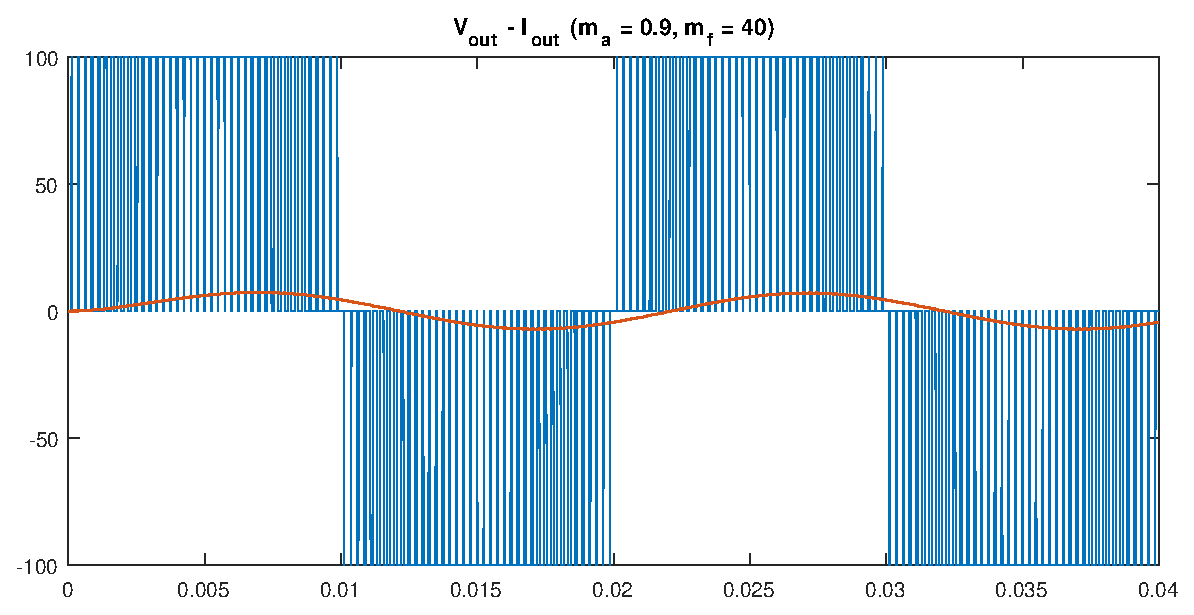
\includegraphics[width=0.95\textwidth]{Images/V_out_I_out_40}
	\end{subfigure}
	\begin{subfigure}{0.49\textwidth}
		\centering
		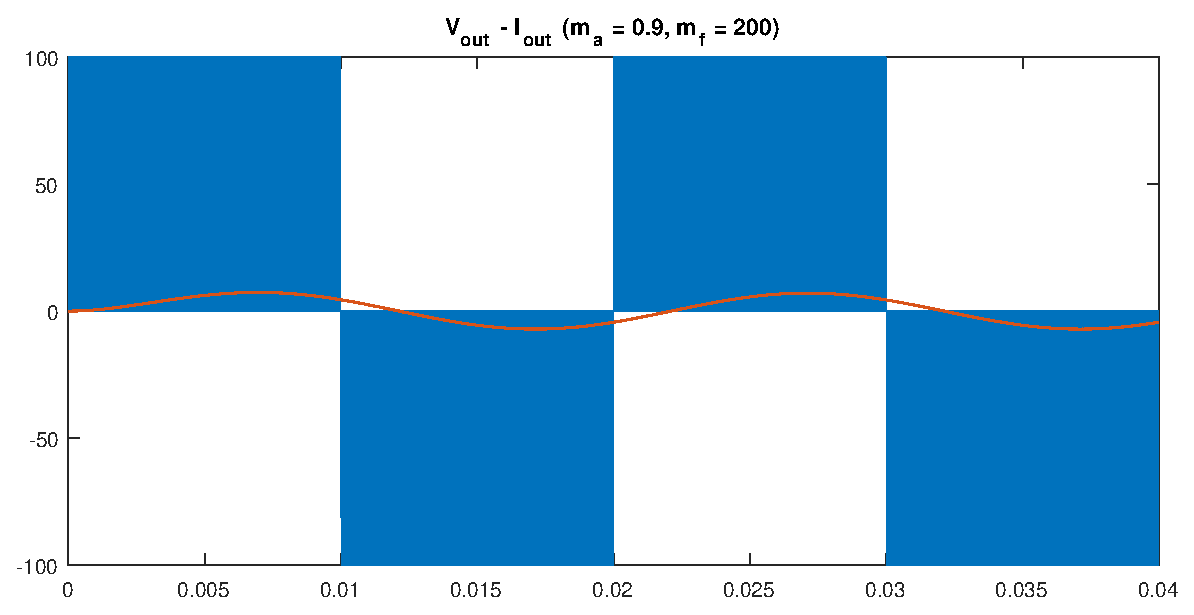
\includegraphics[width=0.95\textwidth]{Images/V_out_I_out_200}
	\end{subfigure}
	\noindent
	Σύμφωνα με τα παραπάνω figures, τόσο η τάση όσο και το ρεύμα εξόδου έχουν την αναμενόμενη μορφή εφόσον το σήμα της τάσης αποτελείται από διακριτούς παλμούς και το ρεύμα εξόδου παρουσιάζει ημιτονοειδή μορφή. Αυξάνοντας τον $m_f$ παρατηρείται ανάλογη αύξηση του αριθμού των παλμών τάσης.  Η συμπεριφορά  αυτή ήταν αναμενόμενη καθώς όπως προαναφέρθηκε στην υποενότητα \ref{single_PWM}, αυξάνοντας τον $m_f$ αυξάνεται ανάλογα η συχνότητα του τριγωνικού παλμού και σε συνδυασμό με την σταθερή συχνότητα του επιθυμητού ημιτόνου. Έτσι, εφόσον οι παλμοί προκύπτουν μέσω σύγκρισης των δύο σημάτων οι παλμοί αυξάνονται.
	\subsubsection*{Ρεύμα εξόδου}
	\begin{subfigure}{0.49\textwidth}
		\centering
		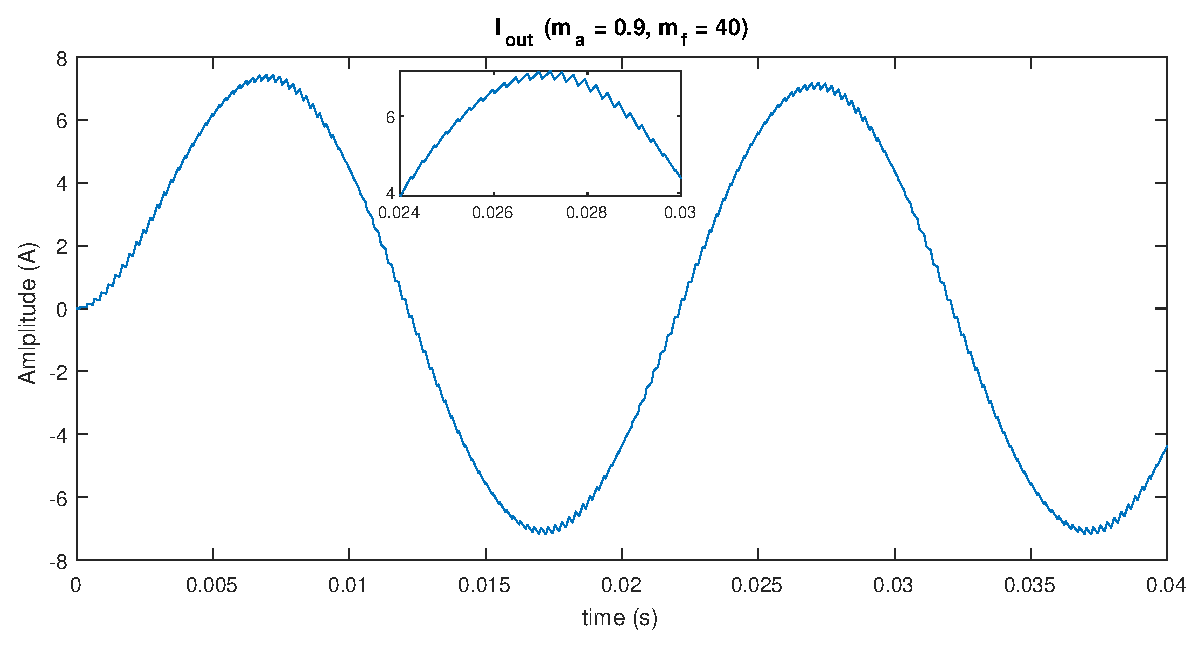
\includegraphics[width=0.95\textwidth]{Images/I_out_40}
	\end{subfigure}
	\begin{subfigure}{0.49\textwidth}
		\centering
		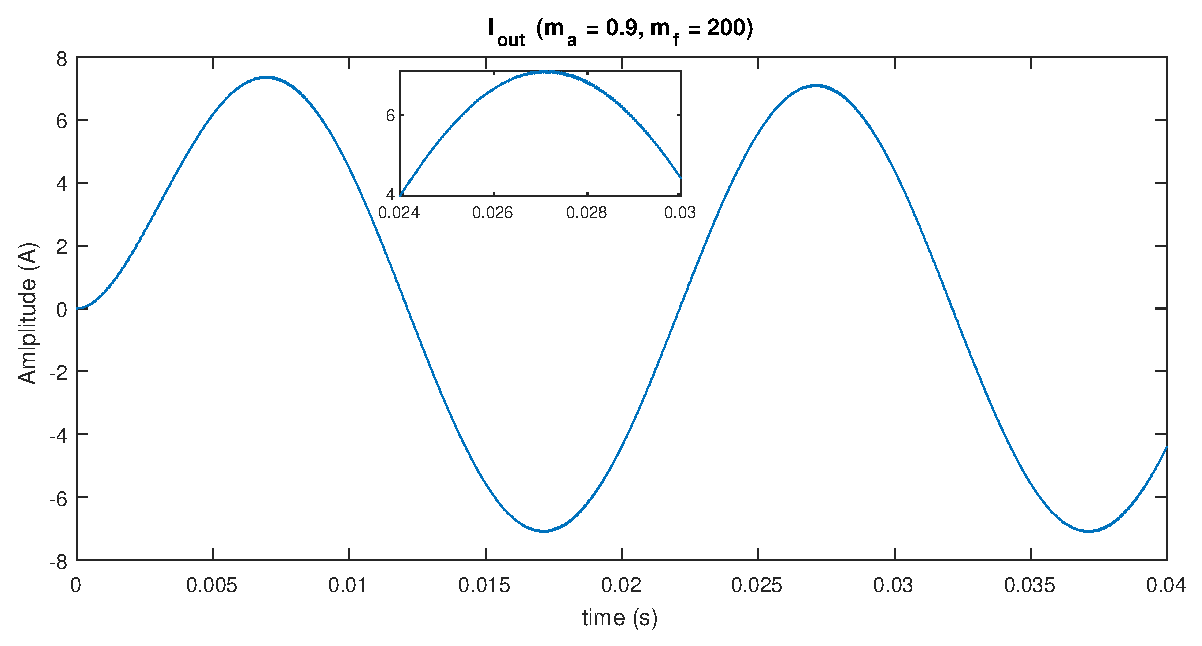
\includegraphics[width=0.95\textwidth]{Images/I_out_200}
	\end{subfigure}
\end{figure}
\noindent
Όσον αφορά το ρεύμα εξόδου παρουσιάζει την αναμενόμενη ημιτονοειδή μορφή. Αυξάνοντας το $m_f$ παρατηρείται μείωση των διακυμάνσεων η οποία συνεπάγεται με μείωση των αρμονικών στο σήμα.\\\\
Η μείωση αυτή οφείλεται εν μέρη στο γεγονός πως το φορτίο είναι ωμικοεπαγωγικό και όπως είναι γνωστό, η σύνθετη αντίσταση του ισούται με $R + j\omega L$, οπότε αυξάνοντας τον $m_f$, αυξάνοντας δηλαδή την συχνότητα του φέροντος, αυξάνεται και η σύνθετη αντίσταση του φορτίου, μειώνοντας  έτσι την επίδραση των ανώτερων αρμονικών. Ο δεύτερος λόγος μείωσης των αρμονικών είναι πως  αυξάνοντας τον $m_f$ οι αρμονικές του σήματος εμφανίζονται σε μεγαλύτερες συχνότητες με αποτέλεσμα να έχουν μικρότερη επιρροή στο σήμα.\\
\clearpage
\begin{figure}[h!]
	\subsubsection*{Τάση Διακοπτικών Στοιχείων}
		\begin{subfigure}{0.49\textwidth}
		\centering
		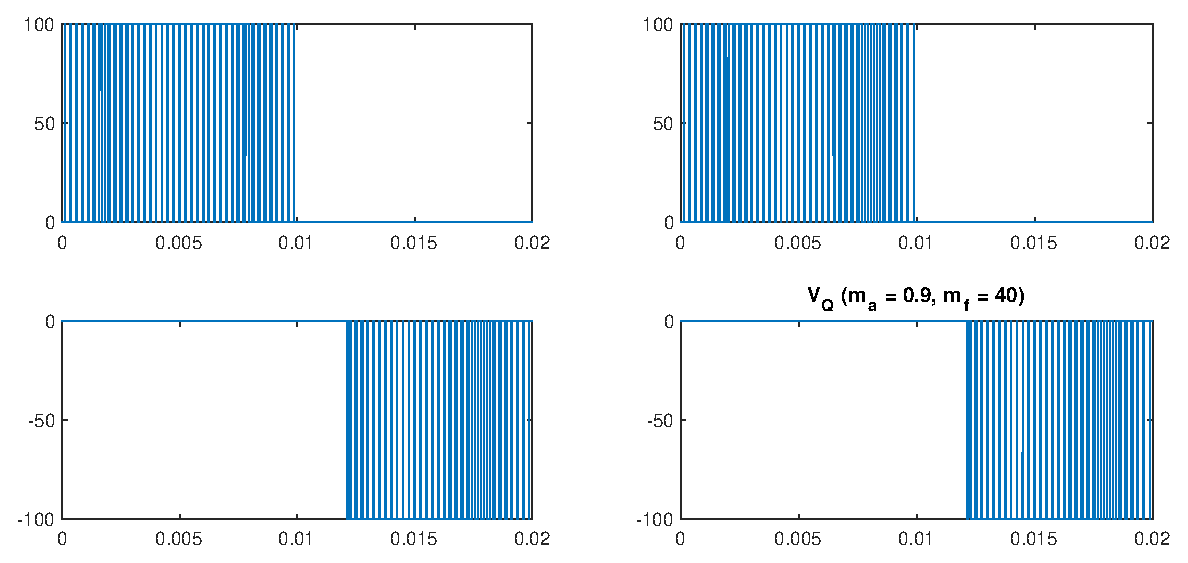
\includegraphics[width=0.85\textwidth]{Images/V_Q_40}
	\end{subfigure}
	\begin{subfigure}{0.49\textwidth}
		\centering
		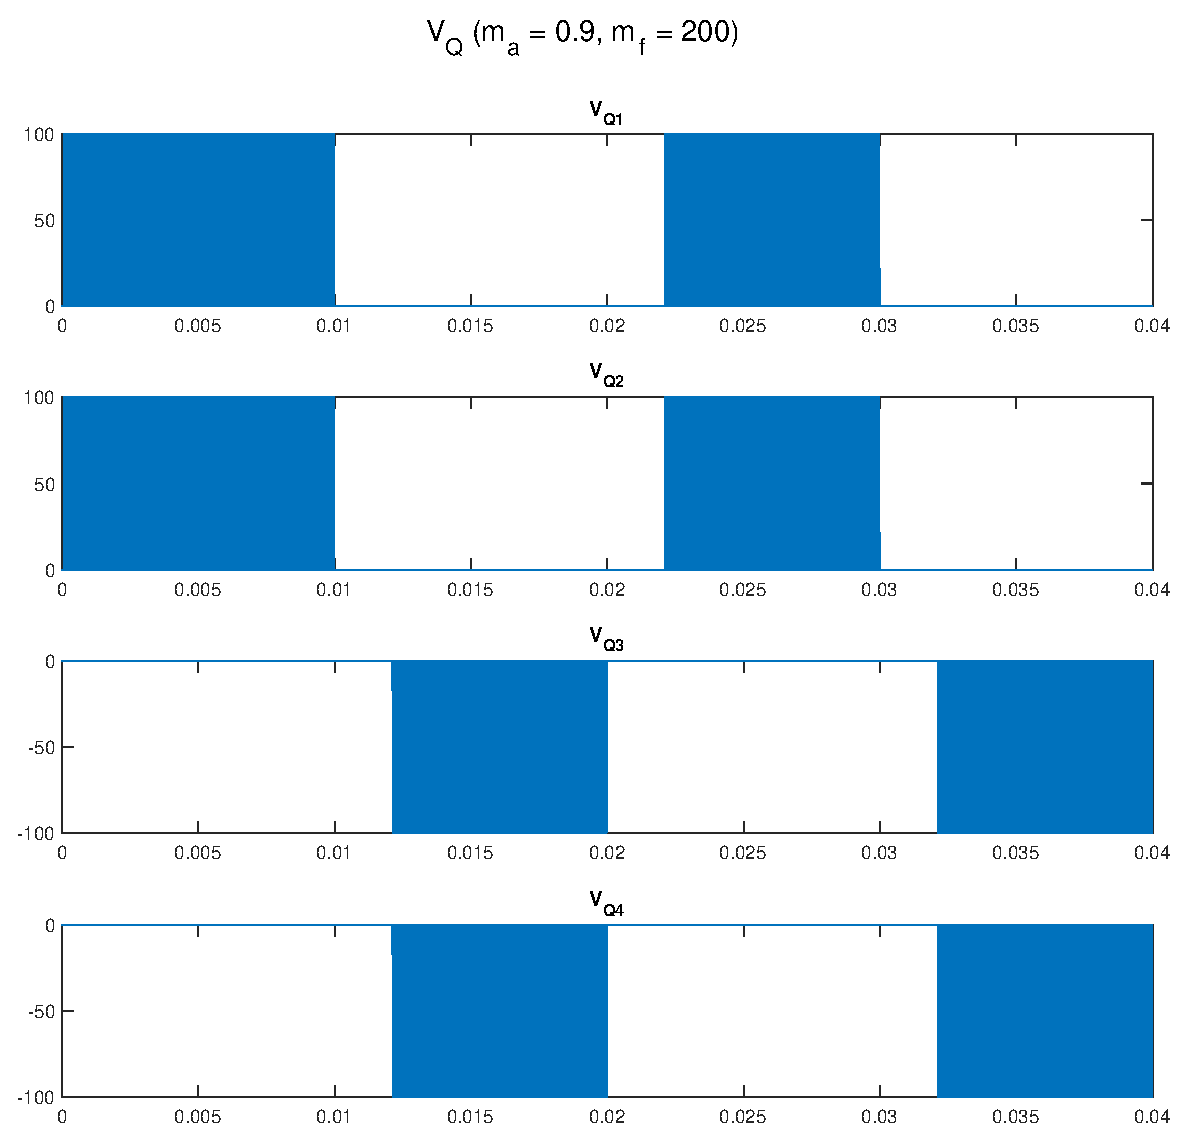
\includegraphics[width=0.85\textwidth]{Images/V_Q_200}
	\end{subfigure}
\end{figure}
\begin{figure}[h]
	\begin{subfigure}{0.49\textwidth}
		\centering
		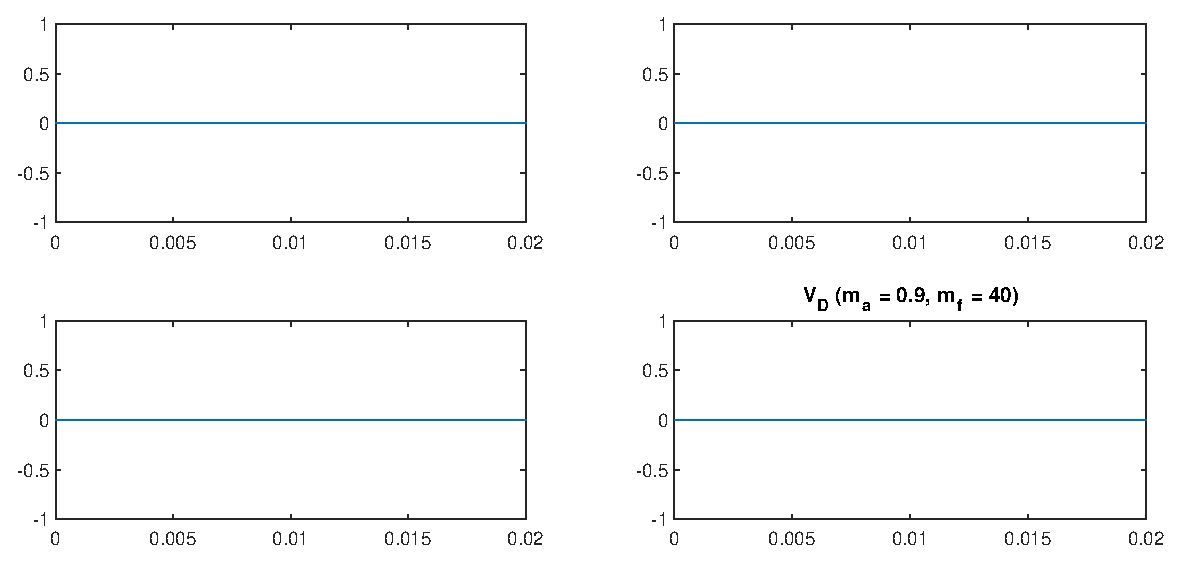
\includegraphics[width=0.85\textwidth]{Images/V_D_40}
	\end{subfigure}
	\begin{subfigure}{0.49\textwidth}
		\centering
		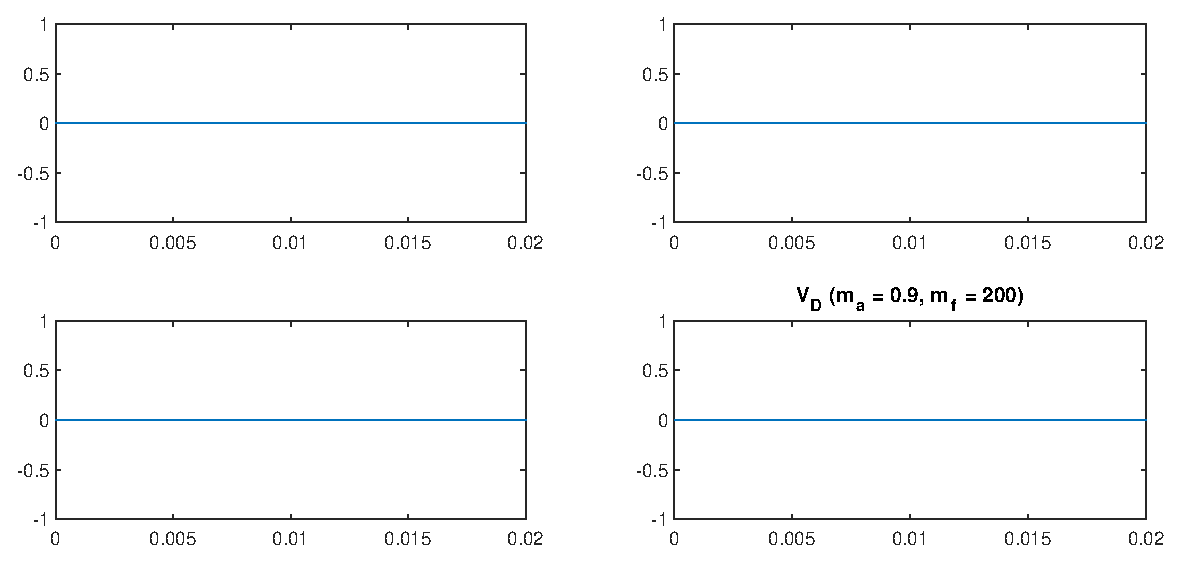
\includegraphics[width=0.85\textwidth]{Images/V_D_200}
	\end{subfigure}
\end{figure}
\noindent
Μέσω της τάσης των transistor, παρατηρείται πως άγουν σε ζεύγη (1-2 και 3-4) όπως ήταν αναμενόμενο καθώς και πως αποτελείται από παλμούς διαφορετικού εύρους. Αυξάνοντας τον $m_f$ παρατηρείται και πάλι πενταπλασιασμός των παλμών. Ακόμα, σε σχέση με τον \textbf{Αντιστροφέα Quasi}, οι παλμοί έχουν τό ίδιο πλάτος. Όσον αφορά τις τάσεις των διόδων, ομοίως με τον μονοφασικό μετατροπέα τετραγωνικού παλμού, είναι ίση με 0 καθώς οι δίοδοι άγουν μόνο στις περιπτώσεις όπου η τάση εξόδου είναι ίση με 0.

\subsubsection*{Ρεύμα Διακοπτικών Στοιχείων}
\begin{figure}[h!]
	\begin{subfigure}{0.49\textwidth}
		\centering
		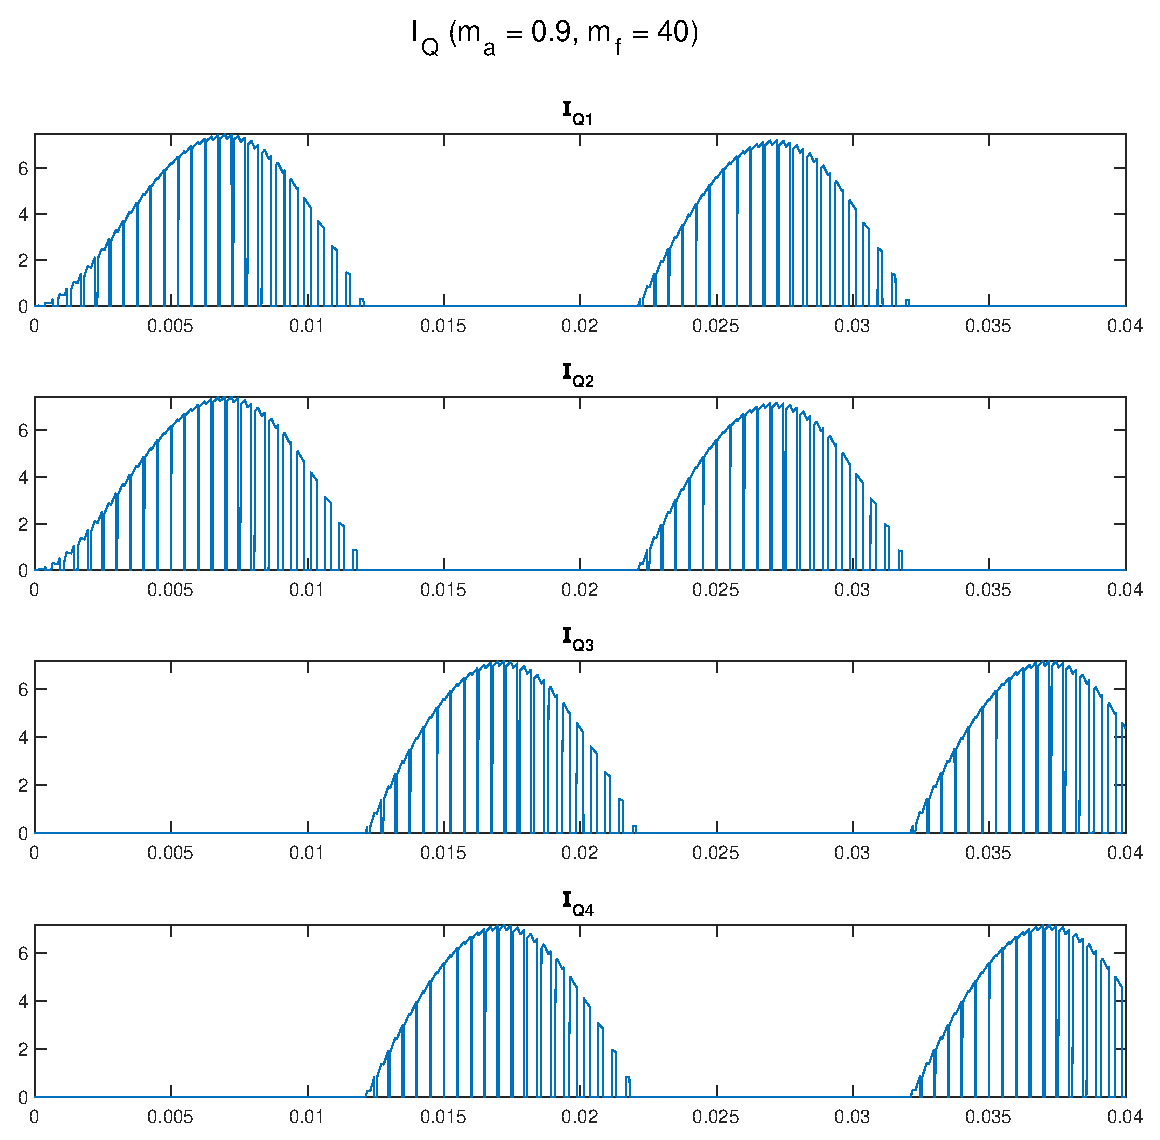
\includegraphics[width=0.8\textwidth]{Images/I_Q_40}
	\end{subfigure}
	\begin{subfigure}{0.49\textwidth}
		\centering
		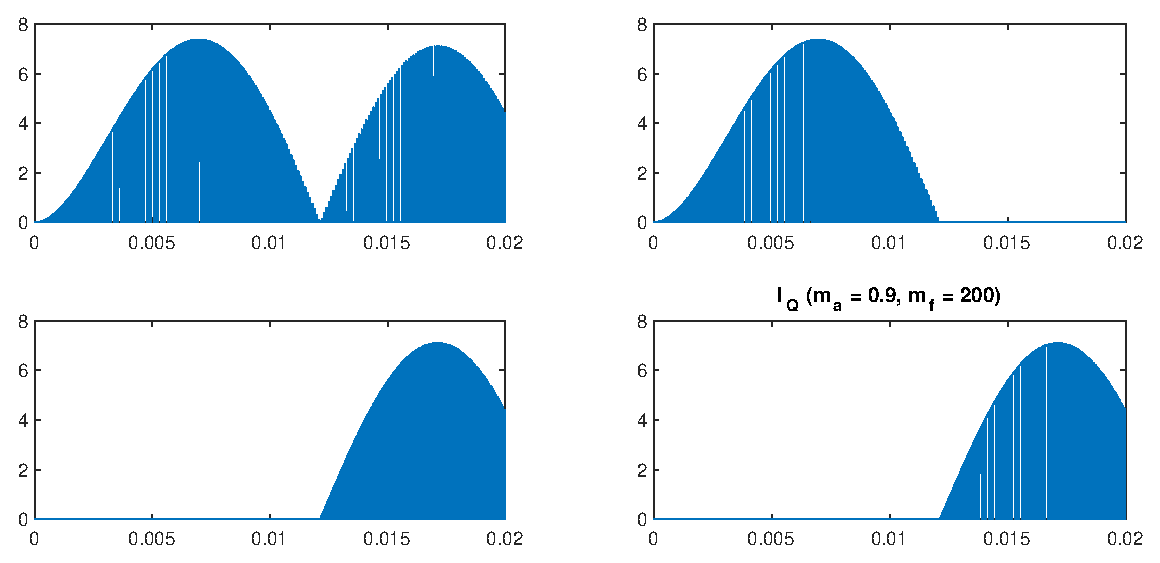
\includegraphics[width=0.8\textwidth]{Images/I_Q_200}
	\end{subfigure}
\end{figure}

\begin{figure}[h]
	\begin{subfigure}{0.49\textwidth}
		\centering
		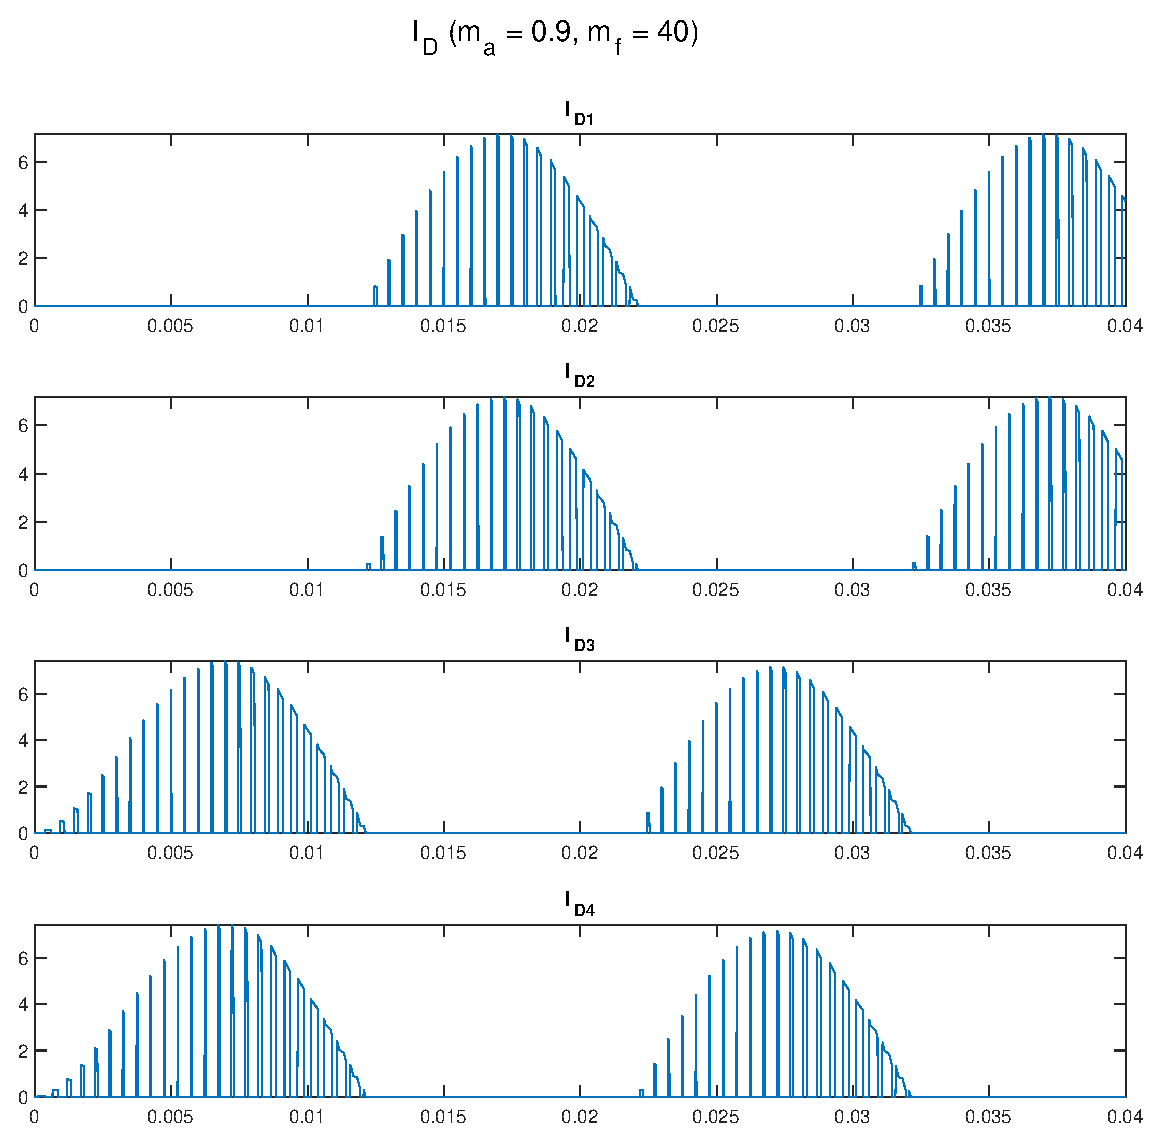
\includegraphics[width=0.8\textwidth]{Images/I_D_40}
	\end{subfigure}
	\begin{subfigure}{0.49\textwidth}
		\centering
		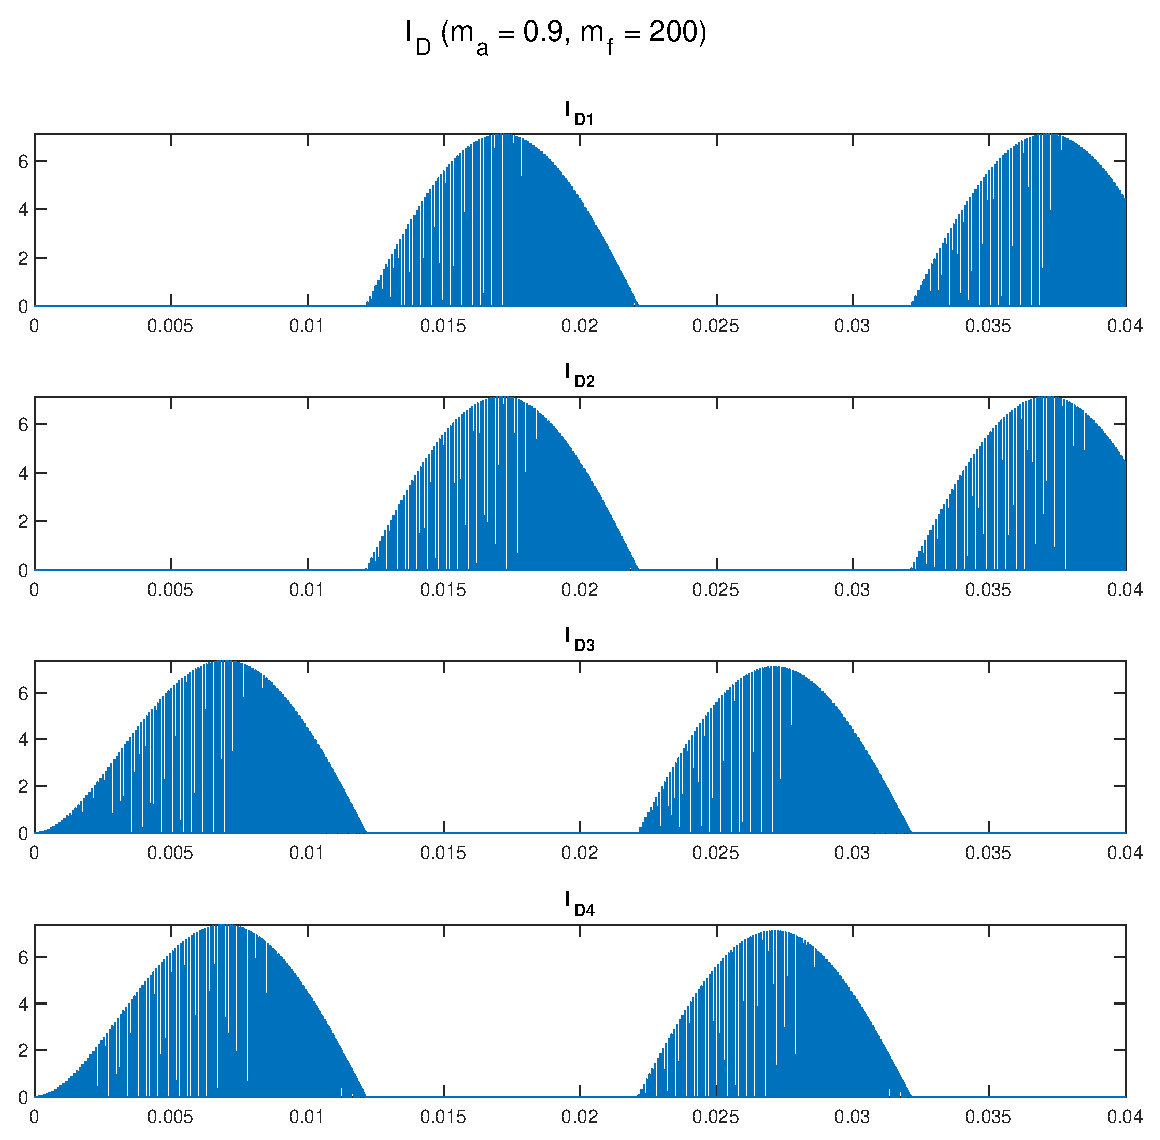
\includegraphics[width=0.8\textwidth]{Images/I_D_200}
	\end{subfigure}
\end{figure}
\noindent
Παρατηρώντας τις κυματομορφές ρεύματος των transistor είναι και πάλι εμφανές πως άγουν σε ζεύγη ανάλογα την φάση λειτουργίας. Επίσης, ομοίως με την τάση, για πενταπλασιασμό του $m_f$ πενταπλασιάζονται οι παλμοί. Ωστόσο, σε αντίθεση με την τάση των διόδων, το ρεύμα δεν είναι μηδενικό αλλά παρουσιάζει όμοια μορφή με το ρεύμα των transistor. Βασική διαφορά μεταξύ των δύο σημάτων είναι πως όταν ρέει ρεύμα μέσω transistor, το ρεύμα της διόδου είναι μηδέν και αντίστροφα ενώ και πάλι για αύξηση του $m_f$, αυξάνεται το πλήθος των παλμών.

\subsubsection*{Ρεύμα Εισόδου}
\noindent\\
Εφαρμόζοντας νόμο ρευμάτων του Kirchhoff, προκύπτει η εξής σχέση για το ρεύμα εισόδου $I_{in}$:
\begin{equation}
	I_{in} - I_{Q_1} + I_{D_1} - I_{Q_3} + I_{D_3} = 0 \xRightarrow{} I_{in} = I_{Q_1} - I_{D_1} + I_{Q_3} - I_{D_3} 	\label{sxesh}
\end{equation}
\begin{figure}[h!]
	\begin{subfigure}{0.49\textwidth}
		\centering
		\includegraphics[width=0.95\textwidth]{Images/2_I_in_40}
	\end{subfigure}
	\begin{subfigure}{0.49\textwidth}
		\centering
		\includegraphics[width=0.95\textwidth]{Images/2_I_in_200}
	\end{subfigure}
\end{figure}\\
\noindent\\
Σύμφωνα με τις παραπάνω γραφικές, παρατηρείται πως το το ρεύμα εισόδου παρουσιάζει εναλλασσόμενη μορφή καθώς παίρνει και θετικές, αρνητικές τιμές και μηδενικές τιμές. Επιπλέον, και εδώ παρατηρείται πως με τον πενταπλασιασμό του $m_f$, πενταπλασιάζεται και ο αριθμός των παλμών.


\clearpage
\subsubsection*{Ισχύς Εισόδου - Εξόδου}
Για τον υπολογισμό της ισχύς απαιτείται γνώση του ρεύματος. Όσον αφορά την έξοδο του κυκλώματος, το ρεύμα είναι γνωστό ωστόσο όσον αφορά την είσοδο, το ρεύμα είναι απαραίτητο να βρεθεί.οπότε εφόσον η ισχύς υπολογίζεται ως το γινόμενο μεταξύ τάσης και ρεύματος, οι ισχύς προκύπτουν ως εξής:
\begin{align*}
	P_{in} &= V_{in} \cdot I_{in} = V_{dc} \cdot I_{in}\\
	P_{in} &= V_{out} \cdot I_{out}
\end{align*}

\begin{figure}[h!]
	\begin{subfigure}{0.49\textwidth}
		\centering
		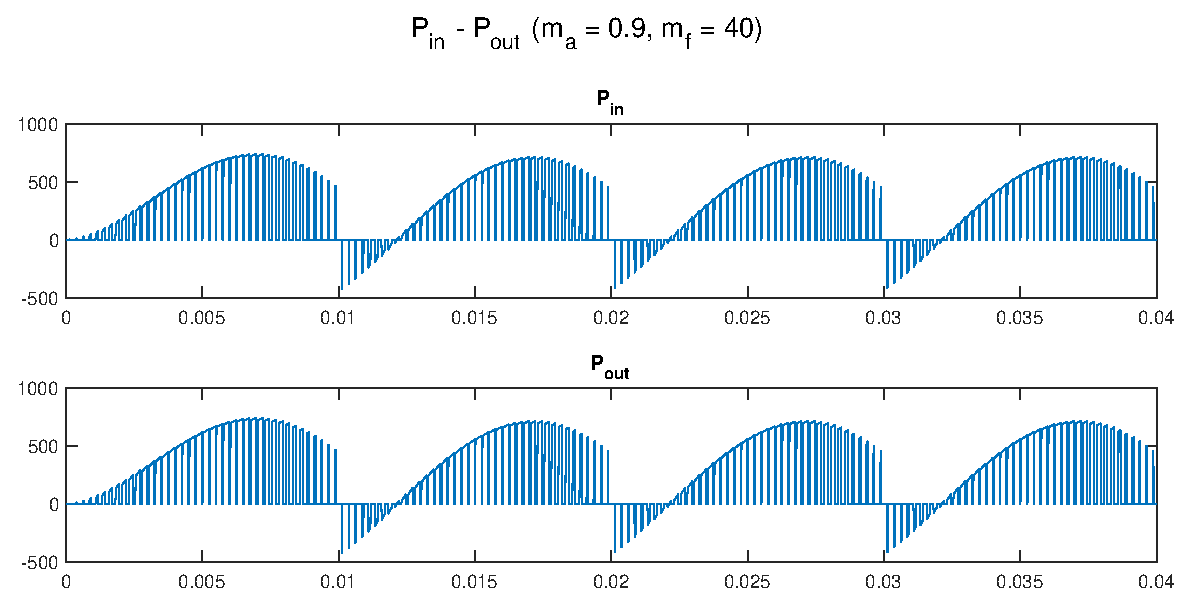
\includegraphics[width=0.95\textwidth]{Images/P_40}
	\end{subfigure}
	\begin{subfigure}{0.49\textwidth}
		\centering
		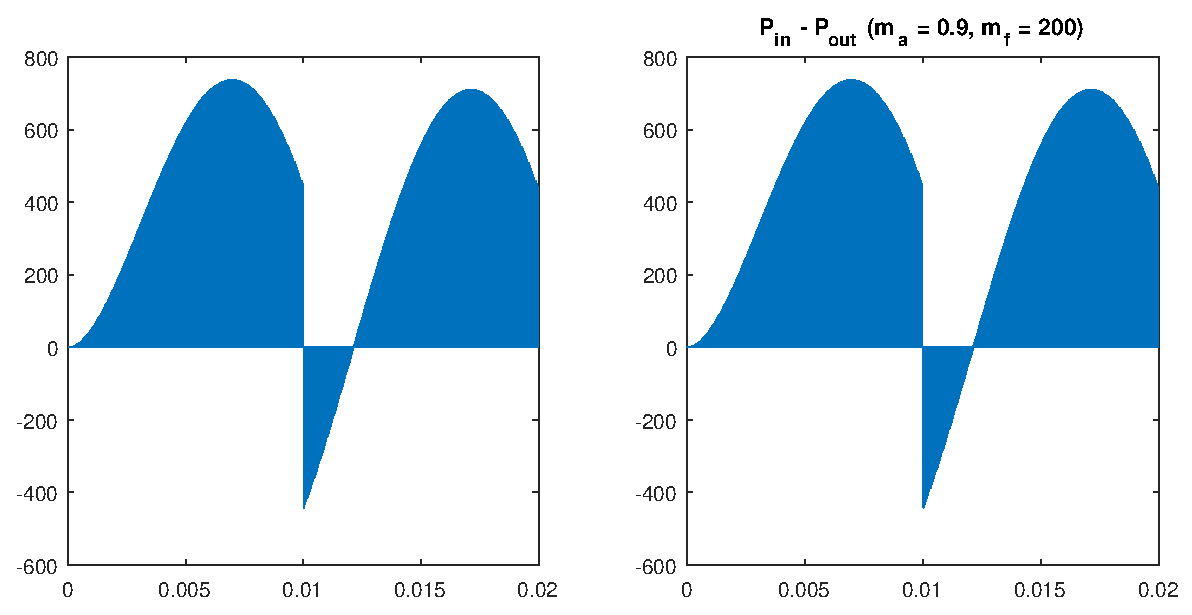
\includegraphics[width=0.95\textwidth]{Images/P_200}
	\end{subfigure}
\end{figure}

\noindent\\
Παρατηρώντας τις κυματομορφές ισχύς εισόδου εξόδου για τις δύο περιπτώσεις, είναι εμφανές και πάλι πως αυξάνοντας τον $m_f$ το πλήθος των παλμών αυξάνεται. Ακόμα, συγκρίνοντας την ισχύ εισόδου με την ισχύ εξόδου κάθε περίπτωσης παρατηρείται πως είναι ακριβώς ίδιες, κάτι το οποίο οφείλεται στην παραδοχή πως οι δίοδοι και τα transistor θεωρούνται ιδανικά και στην Αρχή Διατήρησης της Ενέργειας.

\subsection{Συντελεστής Ισχύος}
Σύμφωνα με την θεωρία ο υπολογισμός του συντελεστή ισχύος υπολογίζεται ως εξής:
\begin{equation*}
	PF = \frac{P}{S} = \frac{I_{out, rms}^2 \cdot R}{I_{out, rms} \cdot V_{out,rms}} =  \frac{I_{out, rms} \cdot R}{V_{out,rms}}  \text{ όπου }	\begin{cases*}
																																														I_{out, rms} = \sqrt{\frac{1}{T} \bigintsss^{T} I_{out} ^2(t)dt}\\
																																														V_{out, rms} = \sqrt{\frac{1}{T} \bigintsss^{T} V_{out} ^2(t)dt}
																																													 \end{cases*}
\end{equation*}

\noindent
Αντικαθιστώντας, προκύπτουν τιμές με πολύ μικρή διαφορά (0.6614 και 0.6617 αντίστοιχα για τις δύο περιπτώσεις) η οποία μπορεί να θεωρηθεί αμελητέα. 
\subsection{Αρμονικές Τάσης Εξόδου}
\noindent
Είναι γνωστό από την θεωρία πως η αρμονικές πέραν της βασικής εμφανίζονται σε συχνότητες με:
\begin{equation}
	f_n = f_s (n \cdot m_f  \pm 1)
\end{equation}

οπότε οι πρώτες αρμονικές (n=1) αναμένεται να εμφανίζονται αρμονικές στις εξής συχνότητες:
\begin{table}[h]
	\centering
	\begin{tabular}{c|cc}
		& $2 \cdot m_f \pm 1$                                         & $2 \cdot m_f \pm 3$                                         \\ \hline
		$m_f = 40$  & \begin{tabular}[c]{@{}c@{}}3950 Hz\\ 4050 Hz\end{tabular}   & \begin{tabular}[c]{@{}c@{}}3850 Hz\\ 4150 Hz\end{tabular}   \\
		$m_f = 200$ & \begin{tabular}[c]{@{}c@{}}19950 Hz\\ 20050 Hz\end{tabular} & \begin{tabular}[c]{@{}c@{}}19850 Hz\\ 20150 Hz\end{tabular}
	\end{tabular}
\end{table}
\noindent\\
Εφαρμόζοντας μετασχηματισμό Fourier στη σήμα της τάσης εξόδου, προκύπτουν οι ακόλουθες κυματομορφές:
\begin{figure}[h!]
	\begin{subfigure}{0.49\textwidth}
		\centering
		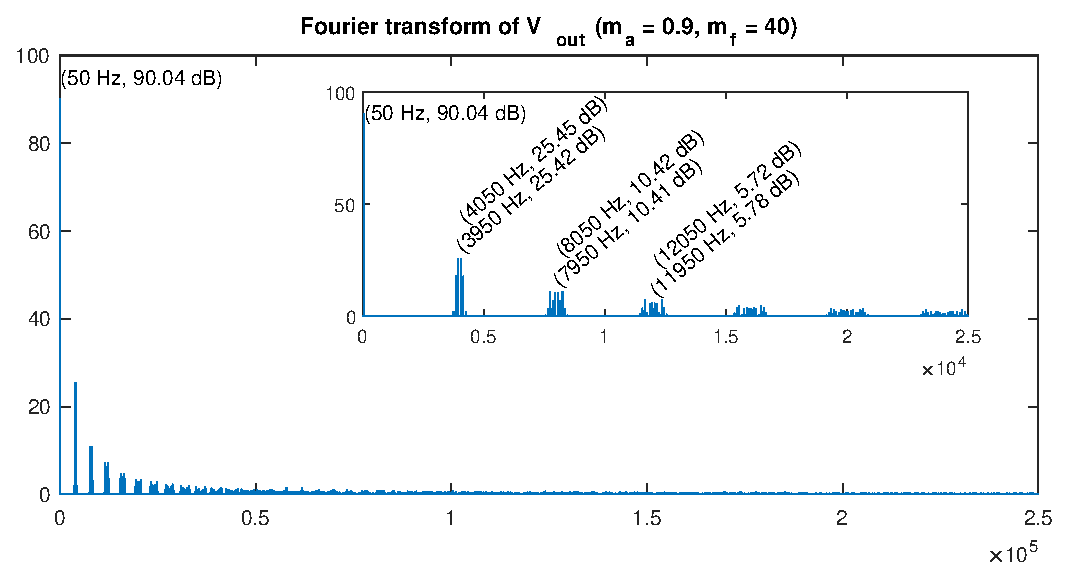
\includegraphics[width=0.95\textwidth]{Images/FV_out_40}
	\end{subfigure}
	\begin{subfigure}{0.49\textwidth}
		\centering
		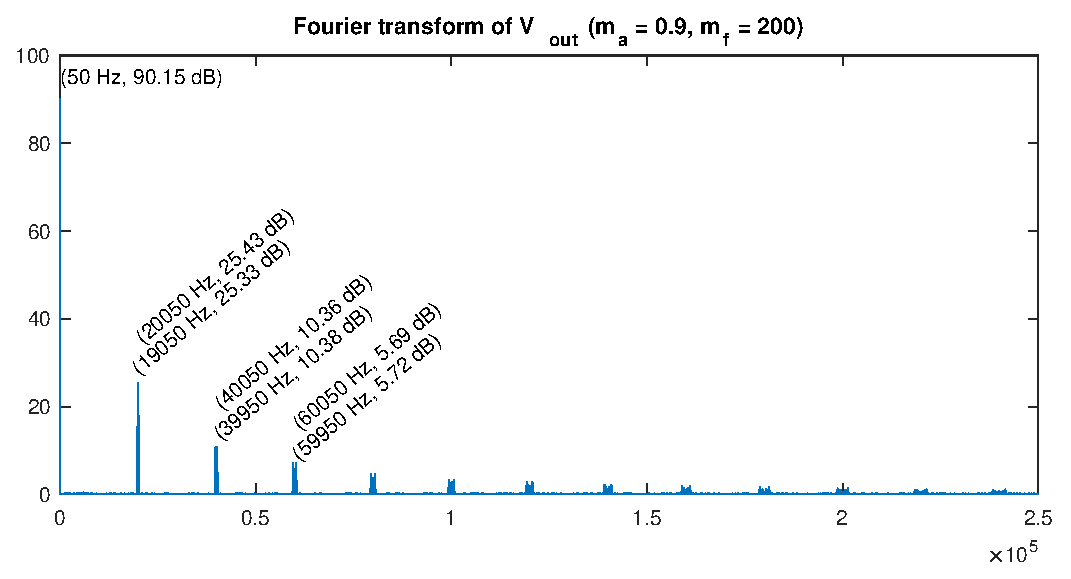
\includegraphics[width=0.95\textwidth]{Images/FV_out_200}
	\end{subfigure}
\end{figure}

\noindent
Παρατηρώντας τις δύο κυματομορφές είναι εμφανές πως οι θεωρητικές τιμές εμφάνισης αρμονικών που εμφανίζονται στο πίνακα συμφωνούν τα αποτελέσματα της προσομοίωσης. Όπως ήταν αναμενόμενο, για πενταπλασιασμό του $m_f$, οι αρμονικές πέραν της βασικής εμφανίζονται σε πενταπλάσιες συχνότητες μειώνοντας έτσι την επίδρασης του στο σήμα εξόδου. Η ιδιότητα αυτή συναρτήσει του ωμικοεπαγωγικού φορτίου το οποίο δρα ως low-pass φίλτρο έχουν ως αποτέλεσμα το σήμα ρεύματος να προσεγγίζει αρκετά αυτό του ημιτόνου, όπως είναι εμφανές παρατηρώντας την αντίστοιχη κυματομορφή. 


	\section{Άσκηση Bonus}
\subsection{Αποδείξτε ότι το πρόβλημα 2023-MaxSAT είναι $\mathcal{N}P$-πλήρες.}
	\noindent
\section{Μη επιλυσιμότητα}

\subsection{Δύο μηχανές Turing M1, M2, υπάρχει έστω και μία συμβολοσειρά για την οποία τερματίζουν και οι δύο μηχανές;}

Για την απάντηση της ερώτησης, μπορεί να χρησιμοποιηθεί το εξής γνωστό πρόβλημα:
\begin{equation*}
	L = \{"M'" : M' \text{ τερματίζει για κάποια είσοδο}\}
\end{equation*}

το οποίο πρόβλημα μπορεί πολύ εύκολα να κωδικοποιηθεί αξιοποιώντας δύο μηχανές Turing:
\begin{equation*}
	L_1 = \{"M_1" "M_2" : \text{$M_1, Μ_2$ τερματίζουν για την ίδια ακριβώς συμβολοσειρά εισόδου} \}
\end{equation*}


\noindent\\
Υποθέτοντας πως το πρόβλημα είναι επιλύσιμο, θα πρέπει η γλώσσα $L_1$ να είναι αναδρομική, οπότε υπάρχει μηχανή Turing $Μ_a$ η οποία αποφασίζει γι αυτή την γλώσσα μέσω της εξής αναγωγής:
\begin{equation*}
	"Μ'" \xrightarrow{} "Μ'""M_2" \text{ όπου η $M_2$ τερματίζει για κάθε είσοδο}
\end{equation*}

\noindent\\
Η διαδικασία εκτέλεσης ξεκινά με την μηχανή M, να υπολογίζει την αναδρομική σχέση $Μ'""M_2"$, δίνει το αποτέλεσμα ως είσοδο στην μηχανή $M_a$ η οποία με την σειρά της δέχεται την συμβολοσειρά $"Μ'""M_2"$ δεδομένου του ότι οι εκάστοτε μηχανές τερματίζουν. Την τελική απόφαση για την γλώσσα την παίρνει η  μηχανή Μ κάτι το οποίο όμως δεν ισχύει άρα, καταλήγουμε σε άτοπο, οπότε το πρόβλημα είναι μη επιλύσιμο.\\



\subsection{Δύο μηχανές Turing M1, M2, τερματίζει η μηχανή M2 για αυστηρά λιγότερες εισόδους από την M1}
Για την απάντηση της ερώτησης, μπορεί να χρησιμοποιηθεί το εξής γνωστό πρόβλημα:
\begin{equation*}
	L = \{"M" : M \text{ τερματίζει για κάποια είσοδο}\}
\end{equation*}

\noindent\\
Αντίστοιχα με την  M, όλες οι "Μ" αναπαραστάσεις ανήκουν στην γλώσσα L και ημιαποφασίζουν για κάποια μη κενή γλώσσα, οπότε το πρόβλημα μπορεί πολύ εύκολα να κωδικοποιηθεί αξιοποιώντας δύο μηχανές Turing:
\begin{equation*}
	L_1 = \{"M_1" "M_2" : \text{$M_1$ τερματίζει για περισσότερες εισόδους σε σχέση με την $Μ_2$} \}
\end{equation*}


\noindent\\
Υποθέτοντας πως το πρόβλημα είναι επιλύσιμο, θα πρέπει η γλώσσα $L_1$ να είναι αναδρομική, οπότε υπάρχει μηχανή Turing $Μ_a$ η οποία αποφασίζει γι αυτή την γλώσσα μέσω της εξής αναγωγής:
\begin{equation*}
	"Μ" \xrightarrow{} "Μ""M_3" \text{ όπου η $M_3$ δεν τερματίζει (infinte loop)}
\end{equation*}

\noindent
Η παραπάνω αναπαράσταση είναι αναδρομική καθώς η $M_3$ χρησιμοποιείται εύκολα σε συνέχεια της M. Αντίστοιχα με την προηγούμενη περίπτωση, η $Μ_3$ δέχεται ως είσοδο την M η οποία με την σειρά της υπολογίζει την παραπάνω αναδρομική σχέση. Στην συνέχεια, αξιοποιώντας την μηχανή $M_a$ με είσοδο $"M"M_3"$ την οποία είσοδο αποδέχεται στην περίπτωση όπου η Μ τερματίζει για περισσότερες εισόδους από την $M_3$. Και πάλι, την τελική απόφαση για την γλώσσα την παίρνει η  μηχανή $Μ_3$ κάτι το οποίο όμως δεν ισχύει άρα, καταλήγουμε σε άτοπο, οπότε το πρόβλημα είναι μη επιλύσιμο.



\end{document}